% Vistas anteriores al ADR-16; conservadas como historia, no se incluyen en el SAD vigente.
\section{Contexto y Alcance}
\label{sec:contexto}

El sistema interactúa con cinco roles de usuario (Cliente, Organizador, Empleado, Administrador y
Supervisor de emergencia) y dos sistemas externos (Pasarela de Pagos y Proveedor de
Notificaciones). La Figura \ref{fig:contexto} muestra el diagrama de contexto (Nivel 1 del modelo
C4).

\begin{figure}[H]
\centering
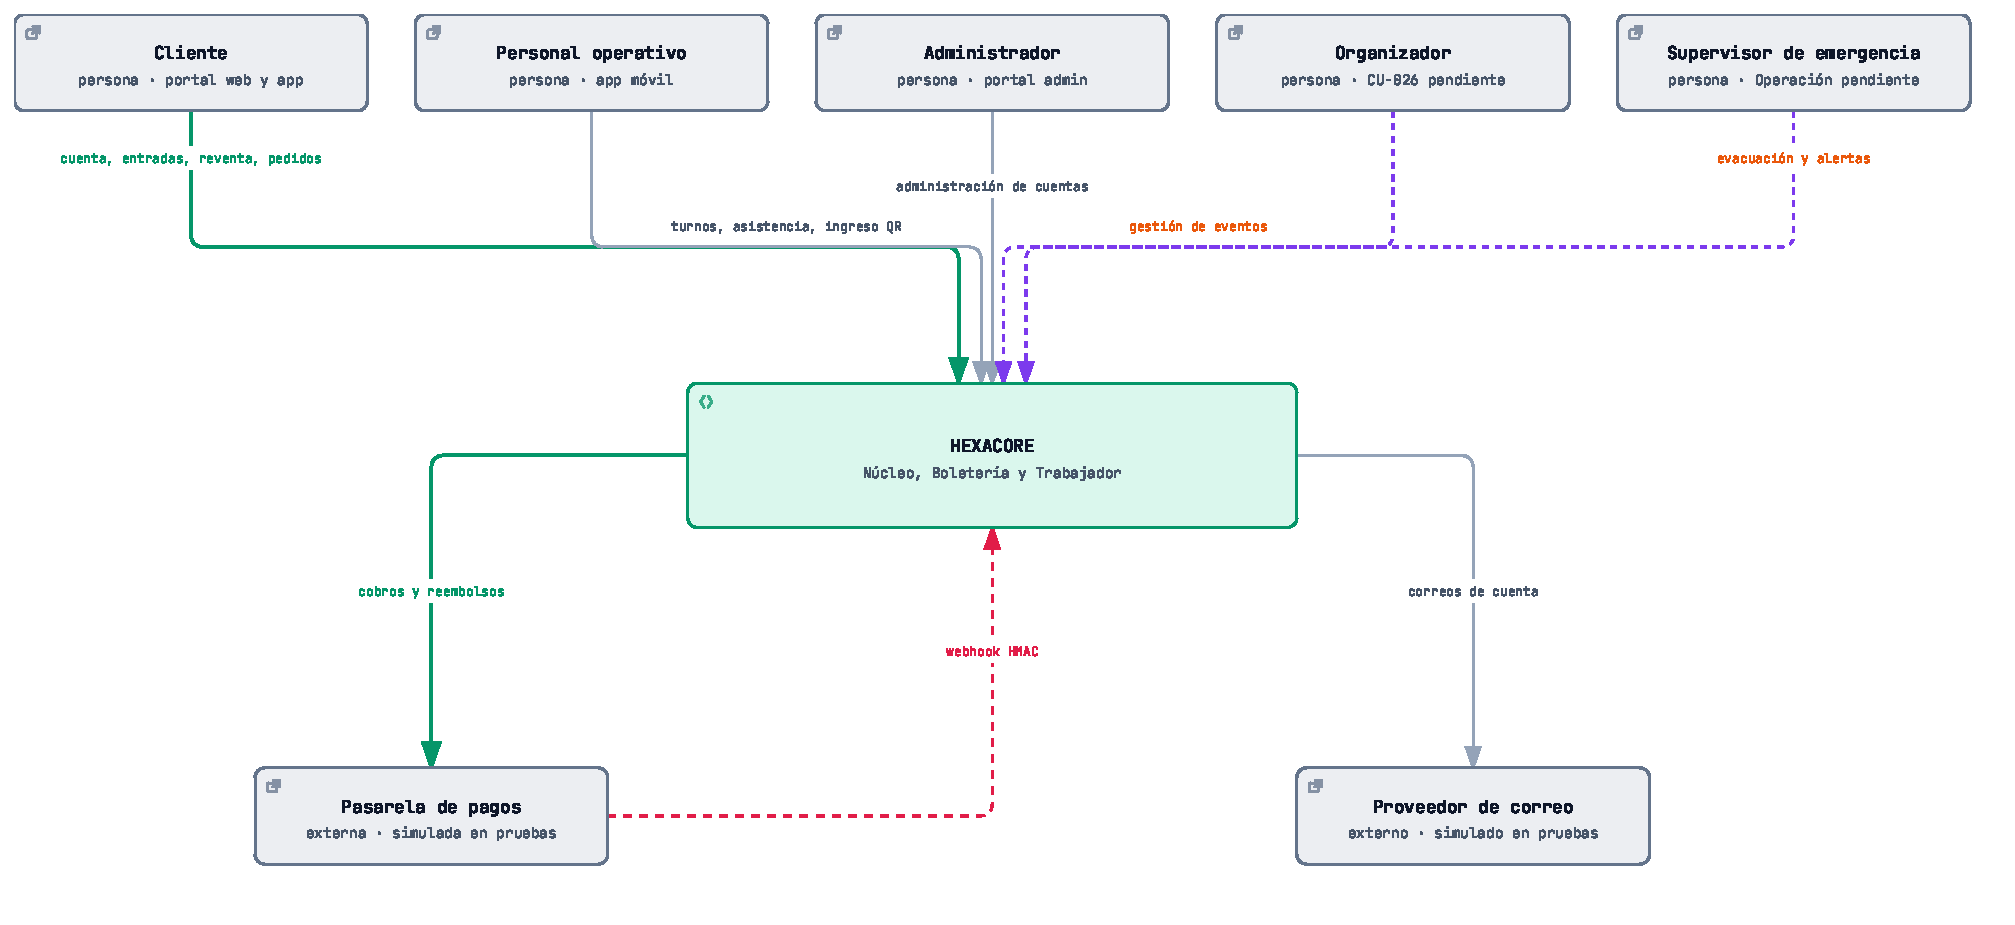
\includegraphics[width=\textwidth]{Diagrams/ArchifyPDF/01-contexto.pdf}
\caption{Diagrama de contexto (Nivel 1, modelo C4).}
\label{fig:contexto}
\end{figure}

\begin{center}
\begin{longtable}{p{3cm}p{3cm}p{6.5cm}}
\toprule
\textbf{Origen} & \textbf{Destino} & \textbf{Descripción}\\
\midrule
Cliente & Sistema & Consulta eventos, compra y revende entradas, reserva parqueadero.\\
Organizador & Sistema & Crea eventos, asigna personal y coordina la operación.\\
Empleado & Sistema & Consulta turnos y registra ingreso/salida.\\
Administrador & Sistema & Administra usuarios, personal y configuración.\\
Supervisor de emergencia & Sistema & Activa y coordina el protocolo de evacuación.\\
Sistema & Pasarela de Pagos & Procesa compras, reventas y reembolsos.\\
Sistema & Proveedor de Notificaciones & Envía notificaciones push, correo y SMS.\\
\bottomrule
\caption{Relaciones del diagrama de contexto.}
\end{longtable}
\end{center}

El diagrama de panorama de sistemas (\textit{System Landscape}, \textit{Diagrams/ArchifyPDF/04-panorama.pdf}
en \textit{C4Diagrams.tex}) amplía este alcance mostrando además cómo el sistema se relaciona con
otros sistemas de la organización (Contabilidad y Facturación, CRM/Marketing y una plataforma de
Analítica), fuera del alcance de este documento pero relevantes para entender el ecosistema
completo.

% ==================== Vista de contenedores ====================
\section{Vista de contenedores}
\label{sec:contenedores}

El sistema se usa desde \textbf{cuatro interfaces}: Portal Web del Cliente, App Móvil del Cliente,
Portal Web Administrativo/Operativo y App Móvil del Personal. Las dos móviles están construidas en
\textbf{Flutter} (ADR-08), lo que permite generar desde una sola base de código los binarios de
Android e iOS. La App Móvil del Personal guarda localmente los QR válidos del evento y las rutas de
evacuación, para validar ingresos y mostrar la evacuación aunque se caiga la red.

El backend son \textbf{catorce servicios} repartidos en dos grupos por el criterio de ADR-14:

\begin{itemize}
\item \textbf{Siete microservicios}, con base de datos propia y réplicas que escalan solas:
      \textbf{Cola virtual}, \textbf{Catálogo} (CU-005), \textbf{Ventas} (CU-001, CU-004),
      \textbf{Pagos}, \textbf{Autenticación} (CU-027, CU-028), \textbf{Acceso QR} (CU-002) y
      \textbf{Notificaciones}.
\item \textbf{Siete servicios de dominio}, que comparten una base central con un esquema por
      servicio y corren redundados pero sin escalar con la demanda: \textbf{Eventos y recintos}
      (CU-026, CU-029), \textbf{Postventa} (CU-003, CU-006), \textbf{Alimentos} (CU-011--015),
      \textbf{Parqueaderos} (CU-021--025), \textbf{Personal y logística} (CU-007--009, CU-016--018,
      CU-030), \textbf{Operación del evento} (CU-010, CU-019, CU-020) y \textbf{Finanzas y
      reportes} (CU-031, CU-032).
\end{itemize}

En total el diagrama tiene \textbf{27 contenedores}: 4 interfaces, el API Gateway, 7 microservicios,
7 servicios de dominio, 5 almacenes de datos, el broker y 2 sistemas externos.

Todos los servicios se exponen por un \textbf{único API Gateway} (ADR-02), que valida el JWT con la
clave pública ---sin llamar a Autenticación en cada petición---, autoriza por el rol del token y, en
la ruta de compra, exige y gasta el turno de la Cola virtual antes de dejar pasar a Ventas
(ADR-15). Entre ellos se comunican de forma asíncrona por un \textbf{broker de eventos}: los
servicios no se llaman en cadena para avisarse de cambios, publican hechos y quien le interese los
consume. Cuando Ventas confirma una compra publica \texttt{Compra\-Confirmada}, y con ese solo
evento Notificaciones manda el QR, Acceso QR lo activa y Finanzas registra el ingreso.

Las llamadas síncronas entre servicios son solo tres, y las tres van hacia quien tiene la
autoridad: Ventas y Postventa piden cobros a Pagos, y Postventa le pide a Ventas cambiar el dueño
de una entrada. \textbf{Acceso QR no llama a Ventas}: valida contra su propia copia de los QR, que
mantiene con \texttt{CompraConfirmada} y \texttt{EntradaActualizada}, así que la puerta sigue
abierta aunque Ventas esté saturada por una apertura de venta. Ventas, a su vez, se entera de qué
entradas se usaron por \texttt{IngresoRegistrado}.

La Tabla \ref{tab:eventos} es el catálogo de eventos del broker. Todo evento que un servicio
publique como consecuencia de escribir en su base sale por una \textbf{bandeja de salida}
(Transactional Outbox, ADR-15): se guarda en la misma transacción que el cambio y un publicador lo
saca al broker después, de modo que ni se pierde si el broker cae ni se publica uno de una
transacción deshecha.

\begin{center}
\begin{longtable}{p{3.4cm}p{2.9cm}p{3.6cm}p{4.4cm}}
\toprule
\textbf{Evento} & \textbf{Lo publica} & \textbf{Lo consumen} & \textbf{Para qué}\\
\midrule
\endhead
\texttt{EventoPublicado} & Eventos y recintos & Ventas, Catálogo & Cargar el inventario y alimentar
el índice de búsqueda\\[0.3em]
\texttt{EventoCancelado} & Eventos y recintos & Catálogo, Ventas, Acceso QR, Notificaciones &
Retirarlo de la búsqueda, cerrar la venta, rechazar en la puerta y avisar a los compradores\\[0.3em]
\texttt{PagoAprobado} / \texttt{PagoRechazado} & Pagos & Ventas & Cerrar o compensar la Saga de
compra\\[0.3em]
\texttt{CompraConfirmada} & Ventas & Acceso QR, Notificaciones, Finanzas y reportes & Activar el QR,
enviarlo y registrar el ingreso\\[0.3em]
\texttt{EntradaActualizada} & Ventas & Acceso QR & Invalidar el QR anterior en una reventa, y
reflejar una entrada en reventa o anulada\\[0.3em]
\texttt{IngresoRegistrado} & Acceso QR & Ventas & Marcar la entrada como usada, para no
reembolsarla (CU-003D) ni revenderla\\[0.3em]
\texttt{AlertaEvacuación} & Operación del evento & Notificaciones & Difundir la evacuación con
prioridad alta\\
\bottomrule
\caption{Catálogo de eventos del broker (ADR-14 y ADR-15).}
\label{tab:eventos}
\end{longtable}
\end{center}

La Figura \ref{fig:contenedores} presenta el diagrama de contenedores.

\begin{figure}[H]
\centering
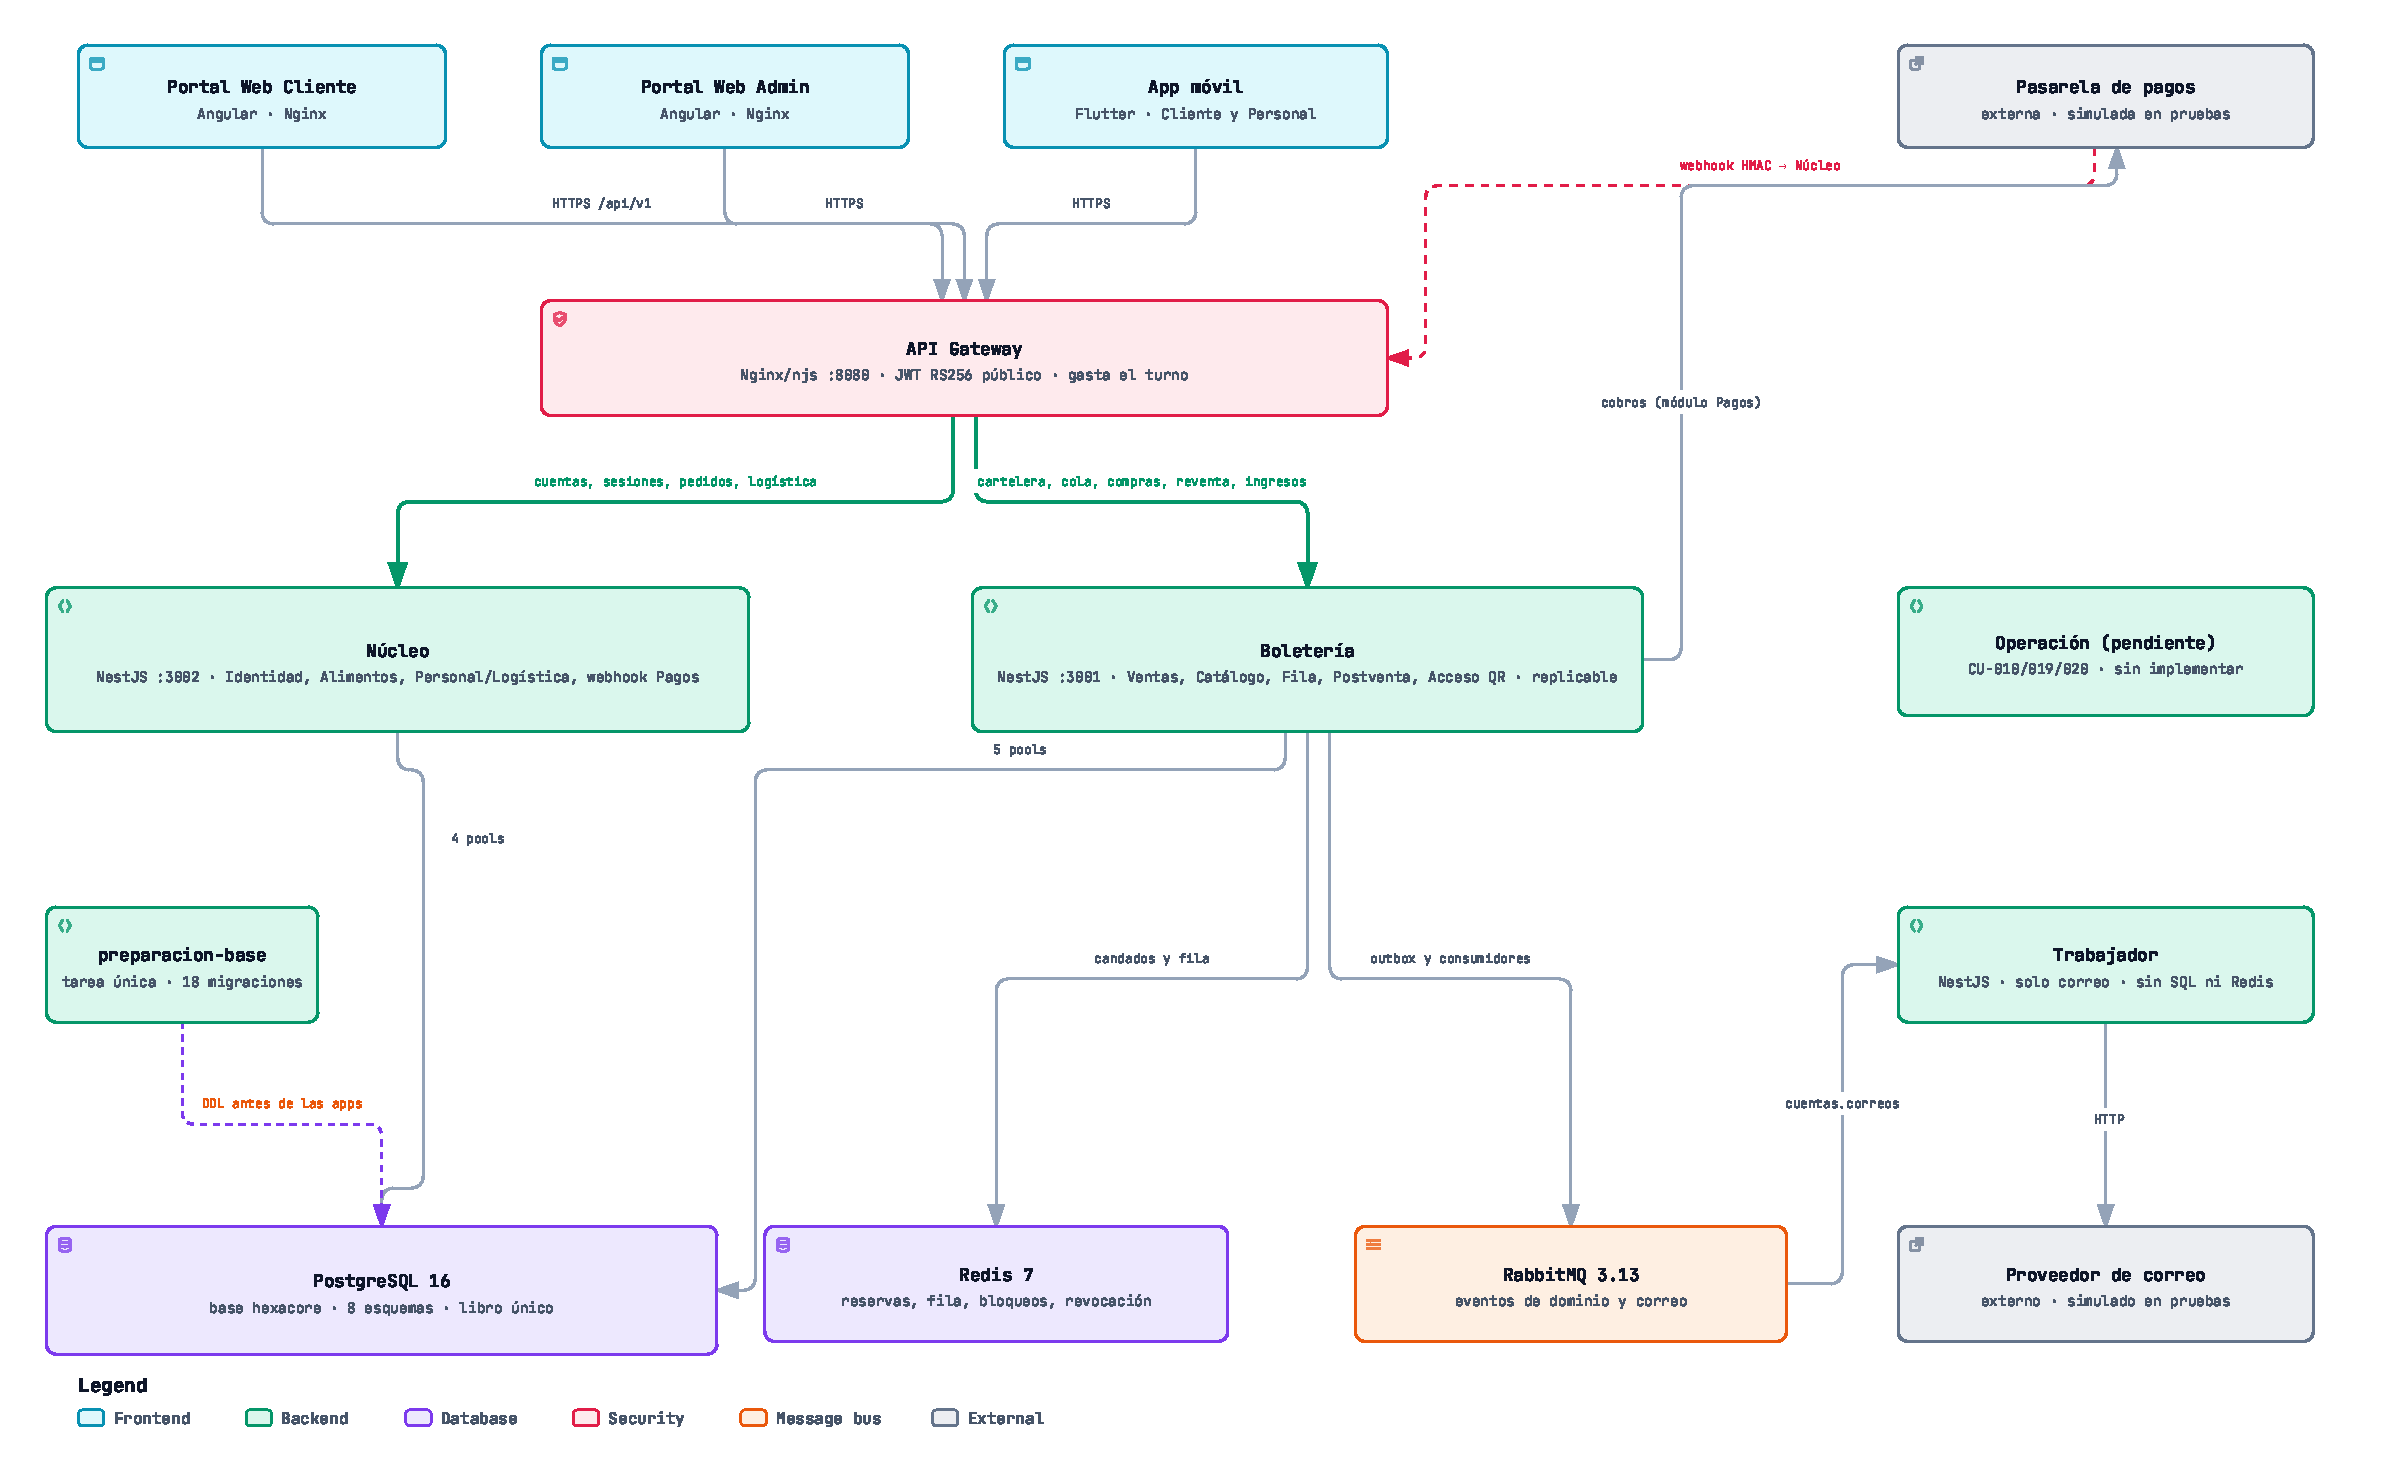
\includegraphics[width=\textwidth,height=0.8\textheight,keepaspectratio]{Diagrams/ArchifyPDF/02-contenedores.pdf}
\caption{Diagrama de contenedores (Nivel 2, modelo C4): siete microservicios y siete servicios de
dominio. Generado con Archify a partir de una especificación JSON; la versión interactiva está en
\texttt{Diagrams/Archify/}.}
\label{fig:contenedores}
\end{figure}

Tres lecturas que el diagrama hace explícitas:

\begin{itemize}
\item \textbf{El camino de compra está completo y aislado.} Cola virtual, Catálogo, Ventas y Pagos
      son los cuatro servicios que el primer ASR obliga a escalar juntos en la apertura de venta, y
      ninguno comparte base con el resto del sistema. La Saga que orquesta Ventas ---reserva
      atómica, cobro idempotente, confirmación o compensación--- recorre exactamente esa franja.
\item \textbf{Los transversales quedan fuera de todo dominio.} Pagos, Autenticación y
      Notificaciones no cuelgan de ningún servicio de negocio: es el segundo criterio de ADR-14, y
      aislarlos es lo que impide que una falla suya degrade varios casos de uso a la vez.
\item \textbf{Los almacenes delatan la división.} Los microservicios apuntan a Redis, al índice de
      búsqueda y a sus bases propias; los de dominio, a la base central. Finanzas y reportes es el
      único que apunta a la réplica de lectura, que es como el sexto ASR impide que un reporte
      pesado degrade la operación durante el evento.
\end{itemize}

La infraestructura de soporte es la misma para los dos grupos:

\begin{itemize}
\item \textbf{Clúster Redis:} el inventario disponible y los bloqueos con vencimiento de Ventas, la
      fila de la Cola virtual, las sesiones de Autenticación y el estado de cada QR.
\item \textbf{Índice de búsqueda:} alimenta las consultas del Catálogo y lo mantienen al día los
      eventos que publica Eventos y recintos.
\item \textbf{Broker de eventos} con tópicos replicados, para no perder hechos si se cae un nodo.
\item \textbf{Servicios externos:} la Pasarela de Pagos ---con la que solo habla Pagos, de modo que
      los datos de tarjeta nunca entran al sistema; su \textit{webhook} de confirmación entra por la
      ruta pública del gateway, firmado--- y el Proveedor de Notificaciones.
\end{itemize}

Para no saturar el dibujo, del gateway solo salen las flechas del camino de compra y la de
Autenticación; en realidad enruta a los catorce. El resto de los servicios sigue el mismo patrón
hacia el almacén que le corresponde y hacia el broker.

\medskip
\noindent\textbf{Estado de implementación.} Corren doce de los catorce servicios sobre Docker
Compose, con las relaciones de ADR-15 ya aplicadas en el gateway, Pagos, Ventas y Acceso QR. Faltan
Eventos y recintos, Parqueaderos y Finanzas y reportes como servicios propios, y con ellos
\texttt{EventoPublicado}, \texttt{EventoCancelado} y la réplica de lectura. El orden para recorrer
esa distancia está en \texttt{Documentation/Work/MIGRACION-ADR-14.md}.

% ==================== Vista de componentes ====================
\section{Vista de componentes}
\label{sec:componentes}

Se detalla el microservicio \textbf{Ventas}, por dos razones. Es el único de los catorce que
cumple los cuatro criterios de extracción de ADR-14 y no solo dos, y es el que orquesta la Saga de
CU-001, que es el mecanismo nuevo que esta arquitectura introduce. La Figura
\ref{fig:componentes} muestra sus componentes internos.

\begin{figure}[H]
\centering
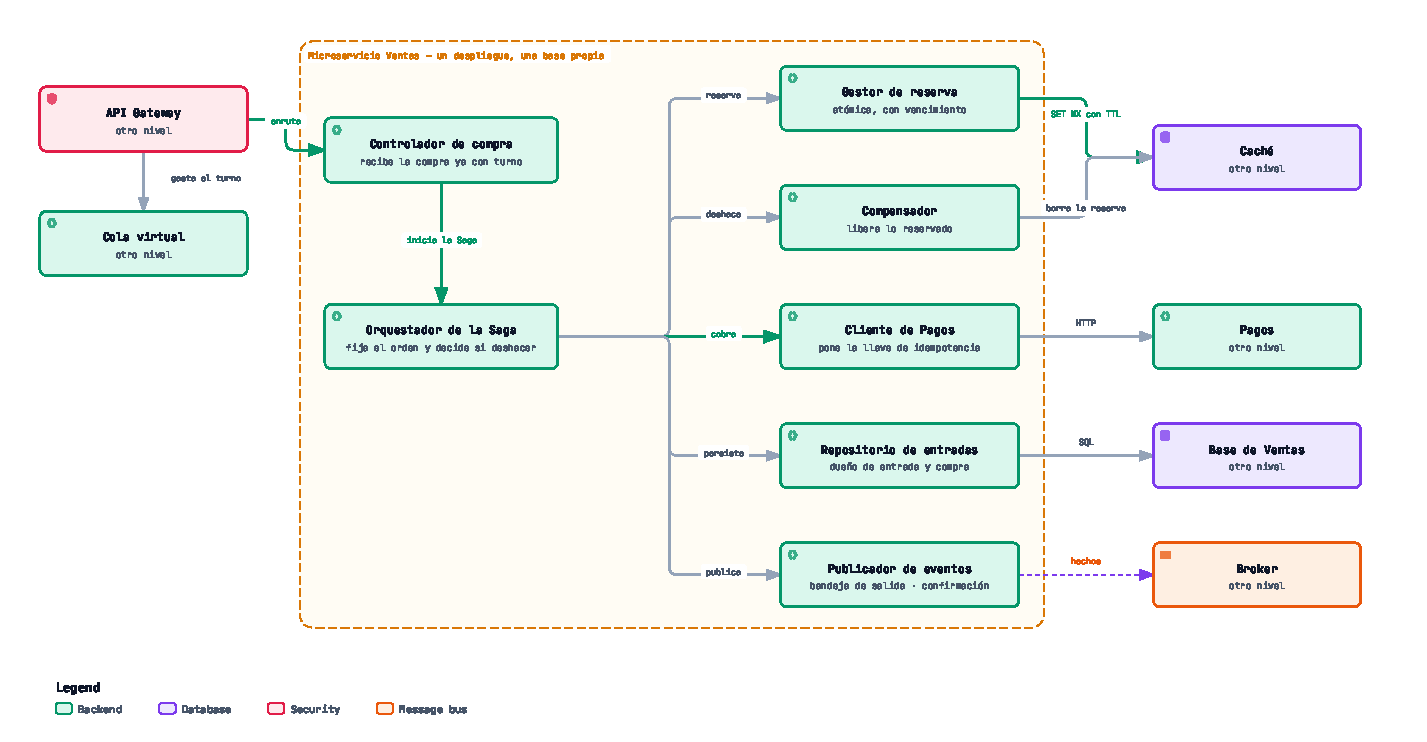
\includegraphics[width=\textwidth]{Diagrams/ArchifyPDF/03-componentes.pdf}
\caption{Diagrama de componentes — microservicio Ventas (Nivel 3, modelo C4).}
\label{fig:componentes}
\end{figure}

El flujo interno es: el \textbf{Controlador de compra} recibe la solicitud enrutada por el API
Gateway y verifica contra la \textbf{Cola virtual} que el token de turno sea válido y no haya
vencido; sin ese token la petición no entra. Delega entonces en el \textbf{Orquestador de la
Saga}, que es quien fija el orden de los pasos y decide si hay que deshacerlos. El Orquestador
pide al \textbf{Gestor de reserva} que aparte las entradas en la caché con una operación atómica
y un vencimiento, encarga el cobro al \textbf{Cliente de Pagos} —que añade la llave de
idempotencia antes de llamar al microservicio Pagos—, confirma la venta mediante el
\textbf{Repositorio de entradas} contra la base propia de Ventas, y anuncia el hecho por el
\textbf{Publicador de eventos} hacia el broker.

El \textbf{Compensador} merece una línea aparte. Es un componente propio y no una rama del
Orquestador porque tiene que poder actuar \emph{sin que nadie se lo pida}: además de deshacer una
Saga que falló, libera por su cuenta las reservas que vencieron porque el comprador abandonó el
proceso. Si fuera una rama del Orquestador, una instancia que muriera a mitad de la compra dejaría
entradas bloqueadas hasta que alguien lo notara.

\medskip
\noindent Dos consecuencias de dónde vive cada dato, que el diagrama hace visibles. El conteo de
entradas disponibles está en la caché y no en la base: es lo que permite reservar de forma atómica
bajo un pico sin que las réplicas compitan por la misma fila. Y la base de Ventas guarda el hecho
consumado —la compra y la entrada con su dueño—, no la reserva en vuelo. Si la caché se cae se
dejan de vender entradas, pero no se venden dos veces: el fallo es cerrado.

\medskip
\noindent\textbf{Estado de implementación.} Estos componentes viven hoy dentro de
\texttt{ventas}, junto a los de Catálogo, Postventa y Acceso QR. El Gestor de
reserva existe (\texttt{gestor-concurrencia.service.ts}) y la llave de idempotencia del Cliente de
Pagos también; el Orquestador y el Compensador no, y por eso hoy no hay un deshacer explícito.

\subsection{Servicio de Personal}

El \textbf{Controlador API} enruta la solicitud hacia el \textbf{Servicio de Asignación de
Personal}, que valida rol, disponibilidad y horario del empleado con apoyo del \textbf{Validador
de Conflictos} antes de confirmar una asignación o un cambio de turno. El \textbf{Gestor de
Turnos} calcula horarios y, junto con el \textbf{Repositorio de Personal}, persiste asignaciones,
turnos y registros de asistencia. El \textbf{Publicador de Eventos} notifica, vía cola de
mensajes, la confirmación de asignaciones y cambios de turno al empleado y al supervisor.

\subsection{Servicio de Eventos / Emergencias}

El \textbf{Controlador API} enruta hacia el \textbf{Servicio de Gestión de Eventos} (CRUD de
eventos, localidades y aforo) o hacia el \textbf{Servicio de Protocolo de Emergencia}, según la
operación. Al activarse una evacuación, este último consulta al \textbf{Gestor de Zonas y Aforo}
(apoyado en Redis para datos de baja latencia) para identificar zonas afectadas, salidas y rutas
disponibles; persiste el incidente mediante el \textbf{Repositorio de Eventos}; y usa el
\textbf{Publicador de Eventos} para difundir alertas y actualizaciones de estado a través de la
cola de mensajes hacia el personal y los asistentes.

\subsection{Servicio de Parqueaderos}

El \textbf{Controlador API} delega en el \textbf{Servicio de Reservas}, que gestiona la reserva
previa y el ingreso/salida de vehículos. El \textbf{Gestor de Ocupación} mantiene en Redis el
estado de ocupación por zona en tiempo real. El \textbf{Procesador de Cobro} invoca la Pasarela de
Pagos para tarifas y reservas. El \textbf{Repositorio de Espacios} persiste las asignaciones, y el
\textbf{Publicador de Eventos} notifica confirmaciones hacia la cola de mensajes.

% ==================== Vista de procesos ====================
\section{Vista de procesos}
\label{sec:procesos}

Se documentan los dos procesos más críticos del sistema desde el punto de vista de los atributos
de calidad: la compra de una entrada (concurrencia y consistencia) y la evacuación ante una
emergencia (disponibilidad y tiempo real).

\subsection{Compra de una entrada con Saga orquestada (CU-001)}

La Figura \ref{fig:secuencia} muestra cómo colaboran los contenedores para resolver una compra.
Es el proceso que mejor explica por qué ADR-14 separa estos servicios: la compra atraviesa cuatro
despliegues distintos —Cola virtual, Ventas, Pagos y el broker— y cada uno tiene su propio
almacén, así que \textbf{no existe una transacción que los abarque a todos}. Por eso el deshacer
tiene que ser explícito, y eso es exactamente lo que es una Saga.

\begin{figure}[H]
\centering
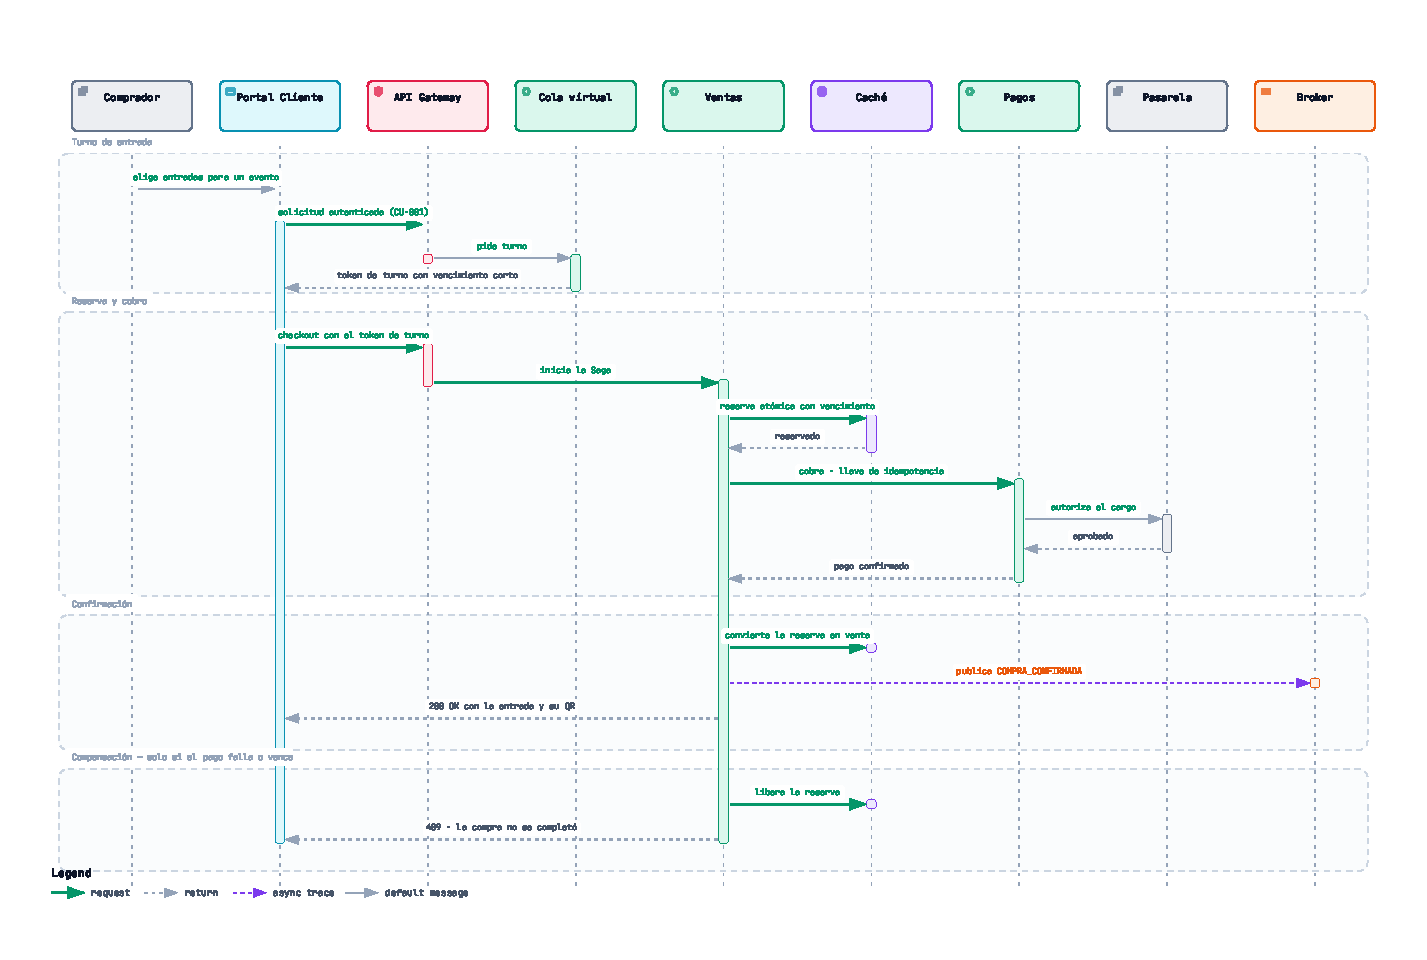
\includegraphics[width=\textwidth]{Diagrams/ArchifyPDF/05-secuencia.pdf}
\caption{Diagrama de secuencia — compra de una entrada con Saga orquestada (CU-001).}
\label{fig:secuencia}
\end{figure}

\begin{enumerate}
\item El comprador elige entradas para un evento; el Portal pide turno a la \textbf{Cola virtual}
a través del Gateway y recibe un token con vencimiento corto. Sin turno no se entra al checkout:
es lo que impide que el pico de una apertura de venta llegue entero a Ventas.
\item El Portal reenvía el checkout con ese token y \textbf{Ventas} inicia la Saga. A partir de
aquí Ventas orquesta: ningún otro servicio decide el orden de los pasos.
\item Ventas aparta las entradas en la caché con una \textbf{reserva atómica con vencimiento}. El
vencimiento es la red de seguridad: si la Saga muere a medias, la entrada vuelve a estar
disponible sola.
\item Ventas encarga el cobro a \textbf{Pagos} con una \textbf{llave de idempotencia}, y Pagos
autoriza el cargo contra la Pasarela. La llave es lo que evita el cobro doble cuando el comprador
reintenta o la pasarela reenvía un \textit{webhook}; una llave reusada con otro pedido se rechaza
en lugar de cobrarse.
\item Con el pago confirmado, Ventas convierte la reserva en venta y publica
\texttt{COMPRA\_CONFIRMADA} en el broker.
\item Ventas responde al Portal con la entrada y su QR. Notificar queda \textbf{fuera del camino
de respuesta}: lo hace Notificaciones al consumir el evento, y si tarda o falla la compra ya está
hecha.
\item \textbf{Compensación.} Si el pago falla o la reserva vence, Ventas libera lo reservado y
responde que la compra no se completó. Es el camino por el que una compra a medias deja de retener
entradas de inmediato, en lugar de esperar al vencimiento.
\end{enumerate}

\medskip
\noindent\textbf{Estado de implementación.} Hoy la compra la resuelve un solo servicio y no hay
orquestación con compensación. Las dos piezas difíciles ya existen —la reserva atómica con
vencimiento, medida en 1 comprador de 50 concurrentes, y las llaves de idempotencia en los dos
caminos de pago—; faltan el orquestador, el deshacer explícito y la cola virtual, que no tiene
código todavía.

\subsection{Evacuación ante emergencias (CU-010)}

\begin{enumerate}
\item El supervisor activa el protocolo de evacuación desde el Portal Web Administrativo,
registrando el tipo y ubicación de la emergencia.
\item El servicio de Eventos/Emergencias identifica las zonas potencialmente afectadas y consulta
el aforo actual, las salidas disponibles y las rutas configuradas.
\item El sistema presenta las rutas y zonas recomendadas; el supervisor confirma el protocolo.
\item Se notifica al personal operativo y se envían instrucciones a los asistentes mediante la
cola de mensajes y el Proveedor de Notificaciones.
\item El sistema monitorea las zonas en tiempo real mientras el supervisor atiende alertas
(ruta bloqueada, zona congestionada, cambio de nivel de emergencia) hasta confirmar la
finalización.
\end{enumerate}

% ==================== Vista física ====================
\section{Vista física}
\label{sec:fisica}

Cada servicio se empaqueta en un contenedor y corre en un \textbf{clúster de Kubernetes}. La
diferencia entre los dos grupos de ADR-14 no está en cómo se empaquetan, sino en \textbf{cómo
escalan}: los siete microservicios tienen autoescalado horizontal (HPA) y los siete servicios de
dominio corren con un número fijo de instancias. La Figura \ref{fig:despliegue} presenta la
topología, con los servicios agrupados por política de escalado.

\begin{figure}[H]
\centering
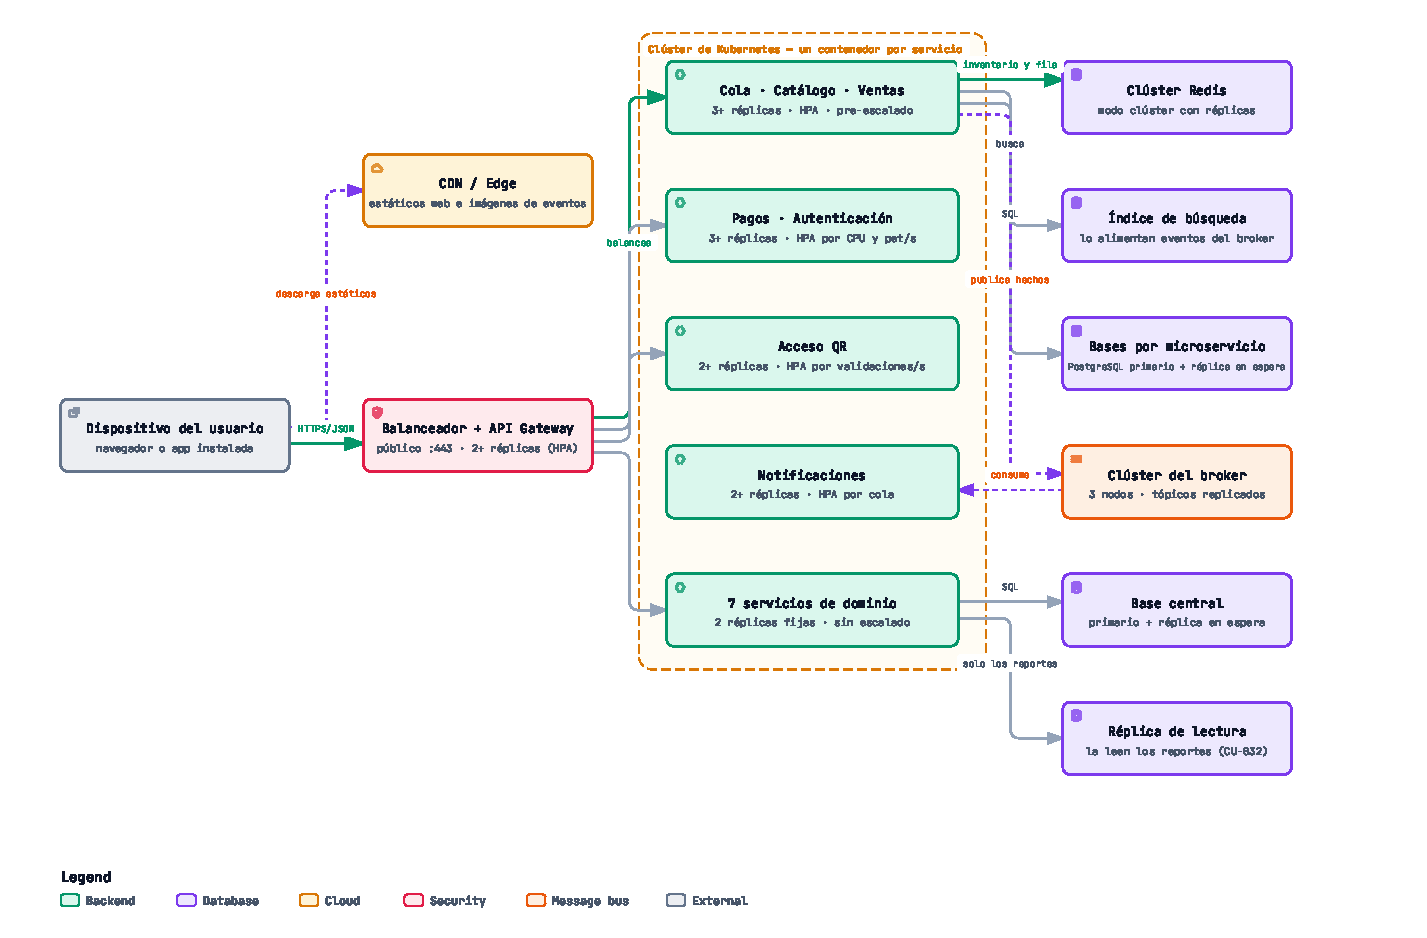
\includegraphics[width=\textwidth,height=0.8\textheight,keepaspectratio]{Diagrams/ArchifyPDF/06-despliegue.pdf}
\caption{Diagrama de despliegue (modelo C4): dos regímenes de escalado sobre un clúster de
Kubernetes. Generado con Archify; la versión interactiva está en \texttt{Diagrams/Archify/}.}
\label{fig:despliegue}
\end{figure}

\begin{center}
\begin{longtable}{p{4.6cm}p{1.8cm}p{3.1cm}p{4.6cm}}
\toprule
\textbf{Componente} & \textbf{Réplicas mínimas} & \textbf{Escalado} & \textbf{Señal para escalar}\\
\midrule
\endhead
Cola virtual, Catálogo, Ventas & 3 & Automático (HPA) & CPU y peticiones por segundo; además se
pre-escalan antes de una apertura de venta anunciada\\[0.3em]
Pagos, Autenticación & 3 & Automático (HPA) & CPU y peticiones por segundo\\[0.3em]
Acceso QR & 2 & Automático (HPA) & Validaciones por segundo en las horas de ingreso\\[0.3em]
Notificaciones & 2 & Automático & Mensajes pendientes en el broker\\[0.3em]
Servicios de dominio & 2 & Fijo & --- (redundancia para disponibilidad)\\[0.3em]
API Gateway & 2 & Automático (HPA) & Peticiones por segundo\\
\bottomrule
\caption{Réplicas y política de escalado por componente. Son valores iniciales propuestos y se
ajustan con pruebas de carga.}
\label{tab:replicas}
\end{longtable}
\end{center}

El pre-escalado de los tres servicios del camino de compra merece el matiz: esperar a que el HPA
reaccione al pico de una apertura anunciada llegaría tarde, porque la señal ---CPU y peticiones por
segundo--- solo sube cuando el pico ya está encima. Notificaciones, en cambio, escala por longitud
de la cola y no por CPU, porque su carga son ráfagas de mensajes pendientes y no uso de procesador.

La infraestructura de datos:

\begin{itemize}
\item \textbf{PostgreSQL} con un servidor primario y una réplica en espera para cada microservicio
      con base propia, y lo mismo para la base central de los servicios de dominio. Finanzas y
      reportes lee de una \textbf{réplica de lectura} de la base central.
\item \textbf{Redis en modo clúster} con réplicas: el inventario de Ventas, la fila de la Cola
      virtual, las sesiones de Autenticación y el estado de los QR.
\item \textbf{Broker con 3 nodos} y tópicos replicados, para no perder eventos si se cae uno.
\item \textbf{CDN} para los frontends web y las imágenes de los eventos, de modo que esas
      peticiones no lleguen al clúster.
\item \textbf{Apps móviles:} consumen el mismo API Gateway que la web. La App Móvil del Personal
      guarda localmente los QR válidos del evento y las zonas y rutas de evacuación, para validar
      ingresos y mostrar la evacuación aunque se caiga la red.
\end{itemize}

Los ambientes de \textbf{desarrollo} y \textbf{pruebas} reutilizan la misma topología a menor
escala: una réplica por servicio (sin autoescalado), sin CDN, y con Redis, el broker y las bases en
un único nodo compartido en vez de clústeres. El de desarrollo se despliega por integración continua
ante cada cambio en la rama principal; el de pruebas se usa para validación \textit{end-to-end} y
pruebas de carga previas a cada entrega, con datos sintéticos que simulan la concurrencia de la
apertura de venta y del ingreso masivo, de forma que los ASR de disponibilidad y rendimiento
(sección \ref{sec:asr}) puedan verificarse antes de producción.

\medskip
\noindent\textbf{Estado de implementación.} El sistema corre hoy sobre \textbf{Docker Compose}, no
sobre Kubernetes, y con los tres servicios de dominio de ADR-12. El paso a esta topología es la
fase F de \texttt{Documentation/Work/MIGRACION-ADR-14.md}.

% ==================== Modelo de datos ====================
\section{Modelo de datos}
\label{sec:datos}

El almacenamiento sigue la misma división que ADR-14 hace de los servicios, y es la parte del diseño
donde esa división se vuelve concreta:

\begin{itemize}
\item Los \textbf{siete microservicios} tienen \textbf{base de datos propia}. Es el tercer criterio
      de extracción: su estado cabe en un almacén separado, así que sus réplicas no compiten por la
      base central. Ventas, Pagos, Autenticación y Acceso QR tienen cada uno su PostgreSQL; el
      Catálogo vive en un índice de búsqueda y la Cola virtual, en Redis.
\item Los \textbf{siete servicios de dominio} comparten una \textbf{base central} con un
      \textbf{esquema por servicio}, que es lo habitual en el estilo basado en servicios. Comparten
      servidor pero no tablas: cada uno escribe solo en su esquema.
\end{itemize}

Las referencias entre servicios ---el propietario de una \textit{Entrada} hacia \textit{Usuario},
que vive en Autenticación--- se resuelven a nivel de aplicación mediante el identificador
correspondiente, y no con llaves foráneas físicas, porque entre bases distintas no existe esa
posibilidad. Dentro de la base central sí podrían existir llaves entre esquemas, pero se evitan por
la misma razón: un servicio que dependa del esquema de otro deja de poder cambiarlo por su cuenta.

A continuación se listan las entidades principales de cada esquema, con sus llaves foráneas lógicas. Las referencias entre dominios (p. ej. el propietario de una
\textit{Entrada} hacia \textit{Usuario}, que vive en el módulo de administración de cuentas) se
resuelven a nivel de aplicación mediante el identificador correspondiente, y no con llaves foráneas
físicas entre bases de datos distintas, lo cual es consistente con la separación de datos
establecida en ADR-01. A continuación se listan las entidades principales de cada esquema, con sus
llaves foráneas lógicas.

\subsection*{Esquema de Entradas / Mercado Secundario}
\begin{itemize}
\item \textbf{Entrada}(id, evento\_id, localidad\_id, propietario\_id, codigoQR, estado)
\item \textbf{PublicacionReventa}(id, entrada\_id, vendedor\_id, precio, estado)
\end{itemize}

\subsection*{Esquema de Personal}
\begin{itemize}
\item \textbf{Personal}(id, usuario\_id, rolOperativo)
\item \textbf{Turno}(id, personal\_id, evento\_id, zona\_id, horario)
\item \textbf{RegistroAsistencia}(id, turno\_id, horaEntrada, horaSalida)
\end{itemize}

\subsection*{Esquema de Eventos / Emergencias}
\begin{itemize}
\item \textbf{Evento}(id, nombre, fecha, categoria, recinto\_id, aforo)
\item \textbf{Recinto}(id, nombre, ciudad, direccion)
\item \textbf{Zona}(id, recinto\_id, capacidad)
\item \textbf{Incidente}(id, evento\_id, tipo, estado)
\end{itemize}

\subsection*{Esquema de Parqueaderos}
\begin{itemize}
\item \textbf{Parqueadero}(id, evento\_id, capacidad)
\item \textbf{EspacioParqueadero}(id, parqueadero\_id, estado)
\end{itemize}

\subsection*{Esquemas de administración general}
\begin{itemize}
\item \textbf{Usuario}(id, nombre, email, credenciales), \textbf{Rol}(id, nombre),
\textbf{UsuarioRol}(usuario\_id, rol\_id)
\item \textbf{Proveedor}(id, nombre, servicio)
\item \textbf{Pago}(id, tipo, monto, estado, referencia\_id, referencia\_tipo) — registra pagos de
Entradas, Pedidos o Parqueaderos mediante \texttt{referencia\_tipo}
\item \textbf{Pedido}(id, cliente\_id, establecimiento\_id, estado, total),
\textbf{Establecimiento}(id, nombre), \textbf{Producto}(id, establecimiento\_id, nombre, precio)
\item \textbf{Reporte}(id, tipo, fechaGeneracion)
\end{itemize}

El motor de base de datos concreto por dominio es \textbf{PostgreSQL} para los esquemas
transaccionales y \textbf{MongoDB} para Reportes (ADR-06).
